\section{Entwicklung des Backends}

\subsection{Einleitung}

Der Umfang dieses Projektes ist die Entwicklung einer Webanwendung zur sicheren Verwaltung von Kundendaten, sicheren Anmeldesystems für Mitarbeiter sowie von Schnittstellen zur effizienten Formularabwicklung im Hintergrund. Dies umfasst auch die Kommunikation zwischen den einzelnen Bereichen der Applikation. Um diese Ziele zu erreichen, wird die Anwendung moderne Technologien und Sicherheitsmechanismen untersuchen und einsetzen, um eine stabile und sichere Plattform zu gewährleisten.
Daraus lässt sich folgende zentrale Forschungsfrage ableiten:
\newline

\begin{center}
    
\textbf{Wie können Formulardaten im Hintergrund einer Webanwendung so verarbeitet werden, dass der Zugriff und die Verwaltung sowohl effizient als auch sicher gestaltet sind?}
\end{center}

Zur Beantwortung wird eine systematische Untersuchung bestehender Backend-Technologien und API-Standards durchgeführt.

\subsection{Backend-Entwicklung}

\subsubsection{Was ist ein Backend?}
Ein Backend ist das Rückgrat jeder Applikation, obwohl es für den Benutzer unsichtbar ist; denn es ist der Teil, der die Daten im Hintergrund verarbeitet und mit der Datenbank interagiert (siehe \cite{wiki-backend}). Es ist dafür verantwortlich, dass die benötigten Daten vom Frontend (also zum Beispiel von einem Formularsystem) richtig und sinngemäß für die Applikation verarbeitet werden. Sowie diese auch, falls notwendig, in einer Datenbank speichert. Umgekehrt ist es aber natürlich auch möglich, dass das Frontend Daten aus der Datenbank benötigt - hierfür stellt das Backend die Brücke zwischen Frontend und Datenbank dar.

\subsubsection{Backend Architektur}

Um nun ein Backend zu entwerfen, muss man eine an die Bedürfnisse des Projekts angepasste Softwarearchitektur, wählen. Hierbei stehen einem zwei populäre Optionen zur Verfügung: die microservice- sowie die monolithische Architektur.

\textbf{Monolithische Architektur}: Diese Art von Architektur ist traditionell am weitesten verbreitet, sowie auch vom Konzept her am einfachsten. Bei dieser Architektur fügt man alle einzelnen entwickelten Komponenten des Programms (z.B. Registrierungs- und Anmelde-Service, die generelle Geschäftslogik, ...) zu einem großen Programm, einem "Monolithen" zusammen. 
Obwohl die Applikation aus kleineren Sub-Modulen besteht, wird sie als eine geplant, entwickelt und letztendlich auch bereitgestellt (\gls{deployment}). Dies hat den Vorteil, dass die Entwicklung, Wartung und das Deployment sich relativ einfach gestalten, da es ja nur eine große Komponente gibt. Jedoch zeichnet sich die monolithische Architektur durch ihre Starrheit sowie fehlende Modularität und Redundanz aus, da, falls eine Änderung an einem Element der Applikation gemacht werden möchte, trotzdem die gesamte Applikation geändert werden müsste (siehe \cite{website-atlassian-microservice-vs-monolothic} und \cite{paper-microservice-vs-monolithic}).

\begin{figure}
  \centering
    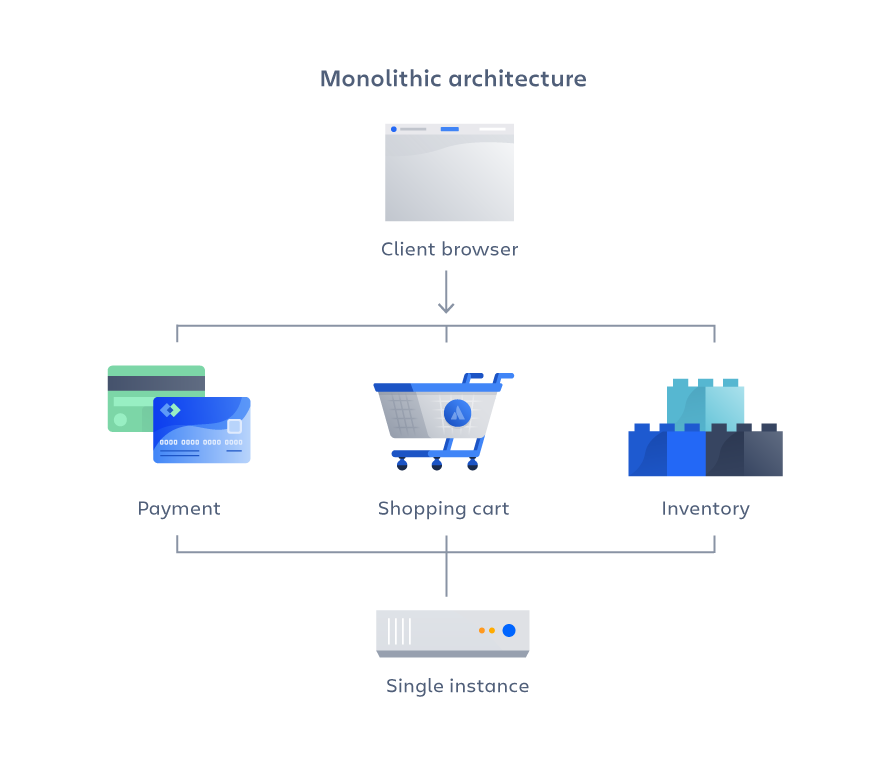
\includegraphics[width=1.0\textwidth]{images/monolithic-architecture-atlassian.png}
   \caption{Grafische Darstellung der monolithischen Architektur. 
   Unabhängig vom konkreten Anwendungsfall, ob jetzt Payment, Shopping Cart oder Inventory, gehören alle Services zu einer Instanz. \cite{website-atlassian-microservice-vs-monolothic}}
   \label{monolithic-arch-atlassian}
\end{figure}

In Abbildung \ref{monolithic-arch-atlassian} lässt sich hierbei erkennen, dass es zwar klar differenzierte Bereiche der Applikation, also zum Beispiel \enquote{Payment}, \enquote{Shopping cart} oder \enquote{Inventory} gibt, diese jedoch trotzdem zu einer einzigen Instanz gehören.

Zusammengefasst bietet eine monolithische Softwarearchitektur also folgende Vorteile:

\begin{itemize}
    \item Leichte Bereitstellung: Nur eine Applikation installieren zu müssen, erleichtert diesen Prozess enorm.
    \item Einfache Entwicklung: Da die Software übergreifend die gleichen Technologien verwendet, gestaltet sich die Entwicklung einfach.
    \item Einfaches Testing: Da die Applikation nur aus einem Teil besteht, lassen sich Tests mit einer höheren Abdeckrate leichter entwerfen.
\end{itemize}

Jedoch bietet diese Architektur auch die folgenden Nachteile:

\begin{itemize}
    \item Langsamere Entwicklung: Eine große, monolithische Applikation verlangsamt die Entwicklung, da der Quellcode immer größer und eventuell komplexer wird und, falls Änderungen in einem Modul getestet werden möchten, muss trotzdem die gesamte Applikation neu gestartet werden.
    \item Erschwerte Skalierung: Applikationen mit einer solchen Architektur können nur schwer großflächig skaliert werden.
    \item Verlässlichkeit und Fehlermanagement: Falls ein Fehler in einem Modul auftritt, könnte dies die restlichen Module der Applikation ebenso betreffen.
\end{itemize}


\textbf{Microservice Architektur}: Diese Softwarearchitektur ist eine relativ neue, jedoch höchst populäre Systemarchitektur. Dieses neue Modell steht laut Google Trends \cite{stats-google-microservice-trend} erst seit 2013 im Fokus, wird seitdem aber immer häufiger auch von Tech-Giganten wie Netflix, Amazon und Co. implementiert.
In der folgenden Grafik kann man das anfangs steigende Interesse sehr gut verfolgen:


\begin{figure}
  \centering
    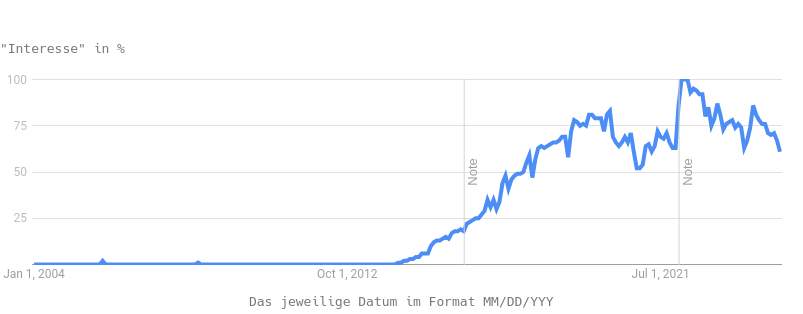
\includegraphics[width=1.0\textwidth]{images/stat-microservice-trend-google.png}
   \caption{Grafische Darstellung des Interesses der Google Benutzer während eines gewissen Zeitraums. \cite{stats-google-microservice-trend}}
   \label{stats-microservice-trend-google}
\end{figure}

Genauer gesagt ist die Microservice-Architektur ein Modell, welches sich auf viele kleine und unabhängige Service, statt eines großen Monolithen verlässt. Jeder dieser Services hat seine eigene Geschäftslogik, Datenbank und verfolgt ein eigenes Ziel.


\begin{figure}
  \centering
    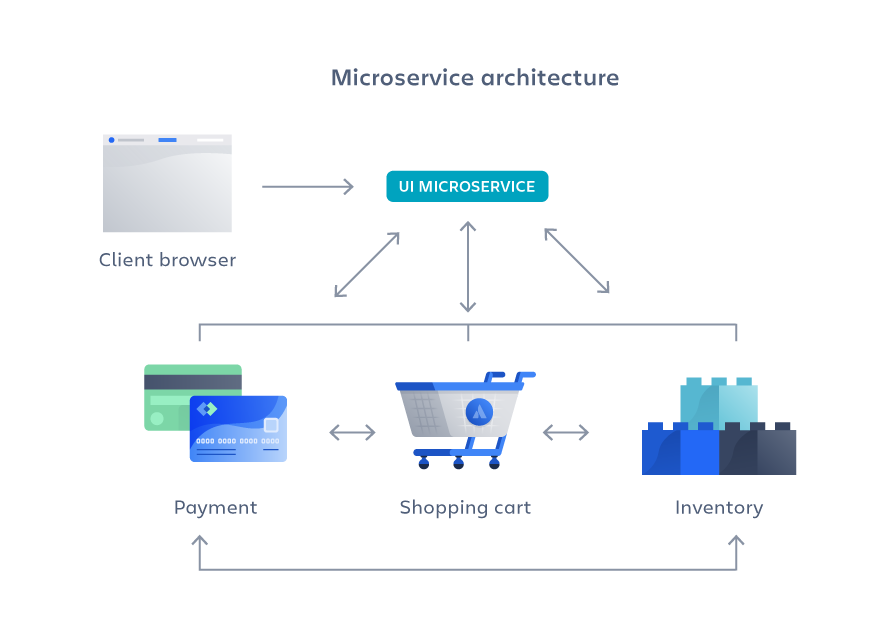
\includegraphics[width=1.0\textwidth]{images/microservice-architecture-atlassian.png}
   \caption{Grafische Darstellung der Microservice Architektur von \cite{website-atlassian-microservice-vs-monolothic}. Der Benutzer greift auf die Benutzeroberfläche zu, welche die einzelnen Services kontaktiert, damit diese dann zusammen die gewünschte Funktionalität ergeben.}
   \label{microservice-arch-atlassian}
\end{figure}

Letztendlich hat die Microservice-Architektur die folgenden Vorteile:

\begin{itemize}
    \item Flexible Skalierung: Wenn ein einzelner Microservice mehr Kapazitäten benötigt, da er vielleicht Ressourcen aufwendigere Aufgaben unternimmt, dann ist dies sehr einfach und kostengünstig möglich.
    \item Schnellere Entwicklung: Im Vergleich zu einer monolithischen Architektur ist die Entwicklung zwar komplexer, jedoch schneller, da Änderungen sofort implementiert und verteilt werden können.
    \item Flexible Wartung / Flexibles Fehlermanagement: Falls ein Service gewartet werden muss, oder möglicherweise ein Fehler bei einem Service auftritt, dann kann das Problem isoliert von den anderen Services behoben werden. Somit hat dies keinerlei Auswirkung auf die restlichen Komponenten der Applikation.
\end{itemize}

Jedoch bringt diese Architektur auch die folgenden Nachteile:

\begin{itemize}
    \item Erhöhte Komplexität: Viele verschiedene Microservices erhöhen die Komplexität einer Applikation und diese können, falls kein Auge darauf geworfen wird, auch komplett durcheinander und unordentlich miteinander kommunizieren. Dies kann sehr schnell sehr verwirrend werden.
    \item Erhöhte Kosten: Ob jetzt in der Entwicklung oder bei dem Deployment (\gls{deployment}); Microservices kosten mehr, da jeder einzelne Service seine eigene Umgebung, seine eigene Datenbank, etc. benötigt.
    \item Mangelhafter Standardisierung: Falls Microservices untereinander, zum Beispiel aufgrund von mangelnder Standardisierung der Protokolle, Schwierigkeiten haben, untereinander oder nach außen zu kommunizieren, erlöschen die meisten Vorteile der Architektur wieder.
\end{itemize}

\subsection{API-Entwicklung}

\subsubsection{Was ist eine API?}

Eine API (\gls{api}), in der deutschen Sprache auch Programmierschnittstelle genannt, ist eine Schnittstelle (\gls{interface}), welche verschiedene Teile einer Applikation miteinander verbindet. Man kann sich das so vorstellen: Wenn man in einem Restaurant speisen möchte, betritt man das Gebäude (in dem Fall: das Frontend). Danach kommt ein Kellner, nimmt die Bestellung auf und liefert diese zum Koch (in diesem Fall: das Backend). Wie hier schnell erkannt werden kann, ist der Kellner derjenige, der das Frontend und Backend miteinander verbindet; die Schnittstelle (siehe \cite{book-api-development-springer}).
\newline

Man unterscheidet hier, laut \cite{book-api-development-springer} S. 4 - 6, in \textbf{Client-API} und \textbf{Server-API}:
\newline


Eine \textbf{Client-API} ist eine Schnittstelle, die es einer Anwendung ermöglicht, mit dem Server zu kommunizieren, oft über HTTP-Anfragen (z. B. REST, GraphQL). Sie wird im Frontend verwendet, um Daten vom Server abzurufen oder zu senden und reagiert in Echtzeit auf Benutzeraktionen.


Eine \textbf{Server-API} hingegen stellt serverseitig Funktionen und Daten bereit, auf die der Client zugreifen kann. Sie verarbeitet Anfragen, führt Logik aus (z. B. Datenbankoperationen) und liefert strukturierte Antworten zurück, die der Client dann verwendet. Sie bildet also das Backend und steuert den Großteil der Geschäftslogik. 

Nun gibt es noch gewisse Standards, welche in der Softwareentwicklung verwendet werden.

\subsubsection{\gls{soap}}

Als das Internet noch am Anfang stand, gab es noch keine richtigen standardisierten Methoden, homogene (\gls{homogen}) Integration von Applikationen zu ermöglichen. 
Denn zu der Zeit liefen die meisten Applikationen im Internet über das \textbf{SOAP} (\gls{soap}), welches ein einfaches Netzwerkprotokoll, verantwortlich für den Austausch von Daten zwischen Systemen sowie Durchführung von RPC (\gls{rpc}), war.

Dieses Netzwerkprotokoll brachte aus der heutigen Sicht einige Nachteile mit sich, welche in \cite{paper-soap} erläutert werden:

\begin{itemize}
    \item Hohe Komplexität: das Protokoll ist sehr komplex, da es auf XML (\gls{xml}) basiert und eine strikte Struktur mit umfangreichen Regeln und Standards erfordert. Dadurch ist die Technologie schwerfällig und kompliziert, sowohl in der Implementierung, als auch in der Wartung.
    \item Overhead: Kommunikationen über SOAP erzeugen viel Overhead, da die Nachrichten viele XML-Tags und umfangreiche Header enthalten. Dies führt zu größeren Datenmengen und damit zu einer langsameren Übertragung.
    \item Aufwendige Integration: Das Protokoll lässt sich nur mit viel Aufwand von modernen Technologien, wie z.B. JavaScript, integrieren, was den Entwicklungsaufwand erhöht.
\end{itemize}

\subsubsection{\gls{rest}}

\textbf{Die Geschichte von REST}

Um nun den älteren \gls{soap}-Standard abzulösen, wurde REST eingeführt. Dieser Standard wurde von Roy T. Fielding in seiner Doktorarbeit Architectural Styles and the Design of Network-Based Software Architectures, siehe \cite{doktorarbeit-rest}, bei der University of Californa im Jahr 2000 erfunden. 


Die REST Architektur ermöglichte es, über das Internet mit jedem Server über das HTTP-Protokoll zu kommunizieren, weshalb man diesen Standard sowohl überall im Internet, als auch im eigenen internen Netzwerk, verwenden kann. 


Als erstes versuchte sich eBay an der Architektur. Nach einem erfolgreichen Gelingen zogen Firmen wie Amazon Web Services, Facebook, Twitter und Google nach. Heutzutage ist es relativ schwierig, eine Applikation ohne REST-API zu finden. Siehe \cite{book-modern-api-development-packt} S. 26.
\newline


 \textbf{Grundlagen von REST}

 Grundsätzlich arbeitet REST mit dem Prinzip, dass alles eine Ressource ist und über einen eindeutigen \gls{url} identifizierbar ist. Dazu zählen z.B. Benutzer, Artikel, etc.

 Da REST ebenso auf dem HTTP-Protokoll basiert, kann man über die folgenden Methoden mit den einzelnen Ressourcen interagieren (siehe \cite{book-modern-api-development-packt} S. 31 - 33):

 \begin{itemize}
     \item \textbf{GET}: Mit dieser Methode lassen sich Daten von der API abrufen. Durch eine URL wie zum Beispiel \textsc{https://server.com/api/user/1} könnte zum Beispiel ein Benutzer mit der id=1 abgerufen werden.
     \item \textbf{POST}: Mit dieser Methode lassen sich über die Schnittstelle neue Daten erstellen. Hier sind die eigentlichen Daten im sogenannten \gls{req-body} untergebracht. Dies kann z.B. eine Anfrage sein, welche ein vom Benutzer ausgefülltes Formular an einen Server sendet.
     \item \textbf{PUT}: Hier können wir bestehende Daten aktualisieren. Das Prinzip ist dasselbe wie bei einer POST-Anfrage, nur mit dem Unterschied, dass eine PUT-Anfrage \gls{idempotent} ist.
     \item \textbf{DELETE}: Mit dieser Methode können Ressourcen auf einem Server gelöscht werden.
 \end{itemize}

Neben den HTTP-Methoden haben \gls{restful-app} fünf Grundprinzipien, welche bei der eigenen Implementierung beachtet werden müssen, um von allen Vorteilen der Architektur profitieren zu können:

\begin{enumerate}
    \item \textbf{Uniform Interface:} Dieses Prinzip gewährleistet eine einheitliche und standardisierte Kommunikation zwischen Client und Server. Es umfasst vier Unterprinzipien (Prompt \cite{prompt-gpt-rest}):
    \begin{enumerate}
        \item \textit{Ressourcenidentifikation:} Jede Ressource wird durch eine eindeutige URI (Uniform Resource Identifier) identifiziert.
        \item \textit{Manipulation durch Repräsentationen:} Clients interagieren mit Ressourcen über deren Repräsentationen, wie JSON oder XML.
        \item \textit{Selbstbeschreibende Nachrichten:} Jede Nachricht enthält ausreichend Informationen, damit der Empfänger sie verstehen und verarbeiten kann.
        \item \textit{\gls{hateoas}:} Clients navigieren durch die Anwendung mittels Hyperlinks, die in den Antworten enthalten sind, siehe \cite{book-modern-api-development-packt} S. 34 - 37.
    \end{enumerate}

    \item \textbf{Cacheable:} Serverantworten sollten Informationen enthalten, die angeben, ob die Antwort vom Client gecacht werden kann. Dies verbessert die Effizienz, reduziert die Serverlast und minimiert die Latenz, indem unnötige Anfragen vermieden werden.

    \item \textbf{Layered System:} Die Architektur ist in Schichten unterteilt, wobei jede Schicht eine spezifische Funktion erfüllt. Clients interagieren nur mit der unmittelbar benachbarten Schicht und sind sich der anderen Schichten nicht bewusst. Dies erhöht die Flexibilität und Skalierbarkeit des Systems.

    \item \textbf{Client-Server}: Dieses Prinzip definiert zwei Aktoren in der Applikation: einen Client und einen Server. Hierbei fragt der Client Informationen vom Server ab (oder möchte eine solche auf dem Server speichern) und tut dies mittels HTTP-Anfragen. Der Server ist dafür zuständig, diese Anfragen vom Client zu empfangen, zu verarbeiten und dem Client eine Antwort zuzusenden.
    \item \textbf{Stateless}: Dies bedeutet, dass, anhand \cite{book-modern-api-development-packt} S. 27, der Server keinen Status von keinem Client  sammelt und verfolgt. Die Anfrage von einem Client muss also alle Informationen beinhalten, welche für das Abarbeiten des Anliegens benötigt werden. Dies verschafft einem bei der Implementierung den Vorteil, dass das System sehr simpel ist; HTTP-Anfragen laufen komplett isoliert voneinander ab.
\end{enumerate}
 

\subsubsection{GraphQL}

\textbf{Die Geschichte von GraphQL}

Vor 13 Jahren, im Jahr 2011, stieß Facebook auf ein Problem: Sie wollten eine performante Mobile Applikation entwickeln, jedoch fehlte ihnen die Technologie dazu. Zu dieser Zeit gab es zwar schon den REST-Standard, jedoch war dieser für die enorme Datenmenge, welche Facebook generierte, einfach nicht ausgelegt. Damals lag die durchschnittliche Internetbandbreite im kB/s-Bereich, weshalb die Firma mit einer performanteren API schnell den Markt erobern würde.

Im Jahr 2012 setzten sich ein paar Facebook-Ingenieure, Lee Byron, Dan Schafer und Nick Schrock, zusammen und entwickelten \textbf{GraphQL}. Rasend schnell breitete sich diese neue Technologie auf die gesamte Firma aus. 

Nach ein paar Jahren der eigenen Verwendung beschloss Facebook, den Quellcode der Technologie für jedermann bereitzustellen. Damit ermöglichten sie die Integration der Softwarearchitektur in sämtlichen bereits bestehenden Technologien, was unter \cite{book-modern-api-development-packt} S. 479 zu finden ist.
\newline

\textbf{REST versus GraphQL im Vergleich}

Grundsätzlich ist GraphQL performanter, flexibler und effizienter als REST.

Denn an sich funktioniert die Architektur so, dass man nicht unzählige \gls{endpoints} für jeden Zweck erstellen muss, sondern die Parameter, welche man von einem Server erfüllt haben möchte, bei einer Anfrage setzen kann.

Möchte man sich jetzt zum Beispiel als Benutzer bei einem Online-Shop anmelden, wobei man nach der Anmeldung zu der Produkt-Seite weitergeleitet wird, ist dies zwar ein Prozess, jedoch müsste man hier bei der REST-Architektur mindestens drei Endpoints implementieren:

\begin{enumerate}
    \item \textbf{Benutzer-Endpoint}: Um die Benutzerdaten zu laden.
    \item \textbf{Produkt-Endpoint}: Um die Produkte zu laden.
    \item \textbf{Einkaufswagen-Endpoint}: Um mögliche Gegenstände aus dem Einkaufswagen des Benutzers zu laden.
\end{enumerate}

All dies ist mit GraphQL nicht notwendig: Hier kann man, anhand der Untersuchung in \cite{book-modern-api-development-packt} S. 480 - 481, dem Server ganz einfach sein Vorhaben schildern, und dieser wird dies dann mit einer Anfrage erfüllen.

\subsubsection{API Sicherheit}

Da diese Schnittstellen elementar für moderne Applikationen sind, stellen sie besonders attraktive Ziele für potenzielle Angreifer dar. Um das Stehlen von Daten und/oder die Übernahme des Servers aufgrund einer Schwachstelle in der Applikation zu verhindern, gibt es gewisse Sicherheitsmaßnahmen, die man setzen kann.

\textbf{Arten von möglichen Angriffen}

Es gibt unzählige Wege, sich selbst Zugang zu einem System zu verschaffen; die beliebtesten sind, laut dem Paper \cite{paper-enterprise-api-security-and-gdpr-compliance} S. 3, die folgenden:

\begin{itemize}
    \item \textbf{Script Insertion}: Eine solche Attacke hat das Ziel, Quellcode auf ein Serversystem zu schmuggeln, mit dem Sinn, dass dieser bösartige Code dann auf diesem System ausgeführt wird. Als Beispiel dafür würde zum Beispiel die Eingabe von JavaScript Quellcode bei einem normalen Formular dienen.
    \item \textbf{SQL injections}: Bei diesem Angriff nutzt der Angreifer ebenso eine Schwachstelle bei der Datenübermittlung an den Server aus. Hierfür muss der Server über eine \gls{sql} Datenbank verfügen. Das Ziel ist es, die Datenbankabfrage so zu verändern, dass zum Beispiel bei der Ausgabe Daten angezeigt werden, die eigentlich nicht abgefragt wurden.
    \item \textbf{Bounds or buffer overflow attacks}: Diese Art von Angriff hat das Ziel, dem Server so viele Daten zu senden, bis das System zusammenstürzt. Hier sprengt die unerwartet große Datenmenge quasi den Rahmen des Systems. 
\end{itemize}

Um diesen Angriffen standhalten zu können und die generelle Sicherheit der eigenen Schnittstelle zu verbessern, kann man folgende Sicherheitsstrategien implementieren (siehe \cite{paper-enterprise-api-security-and-gdpr-compliance} S. 4):

\begin{itemize}
    \item \textbf{Access control management}: Dieser Mechanismus beschäftigt sich damit, den Zugriff der einzelnen Benutzer auf die API zu limitieren. Das heißt, dass man jedem Benutzer einen eindeutigen Schlüssel zuweist, mit dem er sich bei jeder Anfrage ausweisen muss. Somit ist (1) jeder Zugriff auf die API verifizierbar und (2) die Auslastung der Ressourcen unter Kontrolle, da man hier die jeweiligen Benutzer in der Verwendung der Schnittstelle limitieren kann.
    \item \textbf{Client-throttling}: Diese Methode ist ähnlich zum \textbf{Access control management}, bietet jedoch den Vorteil, dass man hier keine registrierten Benutzer benötigt. Hier wird einfach nur jeder Client in der Benutzung der Schnittstelle limitiert. Zum Beispiel kann man dies so konfigurieren, dass jeder Client (z.B. identifizierbar anhand einer IP-Adresse oder einer zugewiesenen temporären \gls{uuid}) die Schnittstelle nur 100-mal pro Minute aufrufen kann. Dies verhindert \gls{ddos} Angriffe.
    \item \textbf{API Gateways Security}: Ein sogenanntes \textit{API Gateway} ist ein wichtiger Bestandteil einer sicheren Schnittstelle. Dieses fungiert als Verkehrspolizei der API Schnittstelle und kontrolliert, ob Anfragen legitim sind, indem es den Benutzer (Autorisierung), den Inhalt und verschiedenste Parameter überprüft. Solch ein Mechanismus verschlüsselt ebenso kritische Daten und verhindert, dass geschützte Daten in System-Logs gelangen. 
    \item \textbf{Communication Security}: Um die Kommunikationssicherheit zu gewährleisten, verwendet man das \gls{tls-ssl} Protokoll. Der TLS Standard wird dazu verwendet, um eine sichere Verbindung zwischen zwei Endpunkten (in diesem Fall dem Client und dem Server) herzustellen. Er stellt sicher, dass jegliche Kommunikation verschlüsselt bleibt. Eine REST-API verwendet HTTP und wird damit von TLS unterstützt.  
\end{itemize}

Diese Mechanismen haben den Sinn und Zweck, den Zugriff auf die API strengstens zu kontrollieren.

\subsection{Ergebnis der Literaturrecherche}

Diese Ausarbeitung verdeutlicht die wesentlichen Prinzipien und Technologien, die für eine erfolgreiche Backend- und API-Entwicklung entscheidend sind. Die Analyse verschiedener Architekturmodelle hat gezeigt, dass die Wahl der richtigen Struktur je nach Projektanforderung maßgeblich zur Effizienz und Skalierbarkeit beiträgt. Ebenso bieten moderne API-Standards wie REST und GraphQL flexible und performante Möglichkeiten, um eine reibungslose Kommunikation zwischen den einzelnen Komponenten zu gewährleisten.
\newline

Die Untersuchung hat auch aufgezeigt, dass die Integration moderner Sicherheitsmechanismen und die effiziente Verarbeitung von Formulardaten im Hintergrund entscheidend sind, um eine stabile und sichere Plattform bereitzustellen. Insgesamt bietet diese Recherche eine solide Basis, um die Entwicklungsziele des Projekts zu verwirklichen und die zentrale Forschungsfrage zu beantworten.